\documentclass[class=report, crop=false, 12pt,a4paper]{standalone}
\usepackage{enumitem}
\usepackage{multicol}
\usepackage{etoolbox}
\AtBeginEnvironment{quote}{\singlespacing\small}
\usepackage{setspace}
\onehalfspacing
\usepackage{graphicx}
\usepackage{float}
\usepackage{amsmath}
\usepackage{amssymb}
\usepackage{siunitx}
\sisetup{detect-all}
\begin{document}
\section{Entropy}
An important inequality that has major consequences in thermodynamics is the \emph{Clausius inequality}.
\[ \oint \frac{SQ}{T} \geq 0 \]
The cyclic integral of \( \frac{SQ}{T} \) is always less than or equal to zero. This inequality is valid for all cycles reversible or irreversible. \( \frac{SQ}{T} \) is the sum of all differential amounts of heat transfer to or from a system, divided by the temperature of the boundary.
\subsection{Proof of the Clausius inequality}
INSERT PROOF
\subsection{The increase of entropy principle}
Consider a cycle. It has two processes:
\begin{itemize}[noitemsep]
  \item Process 1-2: could be reversible or irreversible.
  \item Process 2-1L Internally reversible.
\end{itemize}
The Clausius inequality states:
\[ \oint \frac{SQ}{T} \geq 0 \]
Or,
\[ \int_1^2 \frac{SQ}{T} + \int_1^2\left( \frac{SQ}{T} \right)_{\textrm{int rev}} \geq 0 \]
\[ \int_1^2 \frac{SQ}{T} + (S_1 - S_2) \geq 0 \]
\[ S_2 - S_1 \leq \int_1^2 \frac{SQ}{T} \]
When written in the differential form:
\[ ds \leq \frac{SQ}{T} \]
Where T is the thermodynamic temperature at the boundary. SQ is the heat transferred between the system and surroundings. ds is the differential change in energy. When reversible \( ds = \frac{SQ}{T} \). When irreversible \( ds \leq \frac{SQ}{T} \). This equation shows that:
\begin{quote}
  \begin{center}
    Change in entropy of a closed system during an irreversible process is \emph{always greater} than the integral of \(\frac{SQ}{T}\) evaluated for that process.
  \end{center}
\end{quote}
This inequality shows that during an irreversible process, the entropy  change of a closed system is \emph{always greater} than the entropy of transfer by heat. For a reversible process, \( \Delta S = \int_1^2 \frac{SQ}{T} \), which represents the entropy transfer by heat. Thus, some \emph{entropy generation} must be occurring. This generated entropy is denoted as \(S_{\textrm{gen}}\).
\[ \therefore S_2 - S_1 \geq \int_1^2 \frac{SQ}{T} \]
\[ \therefore \Delta S_{\textrm{sys}} \geq \int_1^2 \frac{SQ}{T} \] 
\[ \therefore \Delta S_{\textrm{sys}} = \int_1^2 \frac{SQ}{T} + S_{\textrm{gen}} \]
\( S_{\textrm{gen}} \) is always positive or zero. This depends upon the process, hence not a property.

When a system is isolated, adiabatic and closed. The heat transfer is zero i.e. \(SQ = 0\).
\[ \therefore \Delta S_{\textrm{sys}} = \Delta S_{\textrm{isolated}} \geq \int_1^2 0 \]
\[ \therefore \Delta S_{\textrm{isolated}} \geq 0 \]
\[ \Delta S_{\textrm{isolated}} = S_{\textrm{gen}} \]
This is the increase of entropy principle. The entropy of an isolated system during a process always increases or in the limiting case of a reversible process, remains constant. Note that in the absence of any heat transfer, entropy change is due to irreversibilities only and their effect is only and always an increase in entropy.

Entropy is an extensive property. Thus, 
\[ \sum^N_{i=1} \Delta S_i = \Delta S_{\textrm{total}} \]
i.e. the use of the change in entropies of the parts of the system is equal to the change in entropy of a system. An isolated system can consist of a number of subsystems. A system and its surroundings, for example, constitute an isolated system since both can be enclosed by a sufficiently large arbitrary boundary at which there is no heat, work or mass transfer. Thus, a system and its surroundings can be considered as two subsystems of an isolated system. Since \( \Delta S_{\textrm{isolated}} = S_{\textrm{gen}} \geq 0 \) but \( \Delta S_{\textrm{isolated}} = \Delta S_{\textrm{total}} = \Delta S_{\textrm{sys}} + \Delta S_{\textrm{surr}} \). Therefore:
\[ S_{\textrm{gen}} = \Delta S_{\textrm{total}} = \Delta S_{\textrm{sys}} + \Delta S_{\textrm{surr}} \geq 0 \]
When considering a reversible process. Then \( \Delta S_{\textrm{sys}} + \Delta S_{\textrm{surr}} = 0 = S_{\textrm{gen}} \). The inequality holds for irreversible process. Note that \( S_{\textrm{gen}}\) can never be negative, but \( \Delta S_{\textrm{sys}} \) can be negative and \( \Delta S_{\textrm{surr}} \) can be negative. The sum of the two must be positive or zero. For example, consider the following system. 
\[ S_{\textrm{gen}} = \Delta S_{\textrm{total}} \]
\[ = \Delta S_{\textrm{sys}} + \Delta S_{\textrm{surr}}\]
\[ = -2 + 3 \]
\[ S_{\textrm{gen}} = 1 \si{\kilo\joule\per\kelvin} \]
\[ S_{\textrm{gen}} = \begin{cases}
  > 0 \textrm{ Irreversible process}\\
  = 0 \textrm{ Reversible process}\\
  < 0 \textrm{ Impossible process}
\end{cases}
\]
\subsubsection{Example question}
Using the increase in entropy principle, show that conduction with finite temperature difference is an irreversible process. 
\[ S_{\textrm{gen}} = \Delta S_{\textrm{total}} = \Delta S_{\textrm{high temp. reservoir}} + \Delta S_{\textrm{low temp. reservoir}} \geq 0\]
\[ \Delta S_{\textrm{total}} = \int \left( \frac{-SQ}{T_H} \right) + \int \frac{SQ}{T_L} \]
\[ = -\frac{1}{T_H} \int SQ + \frac{1}{T_L} \int SQ \]
\[ -\frac{Q}{T_H} + \frac{Q}{T_L} \geq 0 \]
\[ S_{\textrm{gen}} = \frac{-Q}{T_H} + \frac{Q}{T_L} \geq 0 \]
\[ \textrm{since } T_H > T_L \]
\[ \therefore S_{\textrm{gen}} > 0 \rightarrow \textrm{irreversible process} \]
\subsection{Entropy change of pure substances}
The entropy of a pure substance us determined from tables in the same manner as other properties such as volume, internal energy and enthalpy. The value of entropy at a specified state is determined just like any other property.
\begin{itemize}[noitemsep]
  \item Compressed liquids \(\rightarrow\) from tables (if available).
  \item Saturated liquid \(S_P\): from tables.
  \item Saturated mixture: \(S=S_P + xS_{fg}\).
  \item Saturated vapour \(S_g\): from tables.
  \item Superheated vapour: from tables.
\end{itemize}
If the compressed liquid data is not available, the entropy of the compressed liquid can be approximated by the saturated liquid at the same temperature.
\[ S_{\textrm{compressed @ T, P}} = S_{f@T} \]
Note that \( \Delta S = m \Delta S = m(S_2 - S_1)\).
\subsection{T-S diagram characteristics}
Constant volume lines are steeper than the constant pressure lines. Constant pressure lines are parallel to the constant temperature lines in the saturated liquid-vapour mixture region. Constant pressure lines almost coincide with the saturated liquid line in the compressed liquid region. 
\subsection{Isentropic processes}
Entropy can be changed by: heat transfer or irreversibilities. During a process that is internally reversible and adiabatic, the entropy of a fixed mass does not change.
\begin{center}
  Entropy remains constant = isentropic process \(\rightarrow \Delta S = 0 \textrm{ or } S_2 = S_1 \)
\end{center}
\begin{center}
  A reversible adiabatic process \(\rightarrow\) isentropic
\end{center}
\begin{center}
  However, isentropic \(\rightarrow\) reversible adiabatic (Which usually means an internally reversible, adiabatic process)
\end{center}
\subsection{Property diagrams involving entropy}
Two diagrams commonly used in the second-law analysis are the temperature-entropy and the enthalpy-entropy diagrams. Remember:
\begin{align*}
  \frac{SQ_{\textrm{int rev}}}{T} &= dS\\
  \therefore SQ_{\textrm{\textrm{int rev}}} &= TdS\\
  \therefore Q_{\textrm{int rev}} &= \int_1^2 T dS \ (\si{\kilo\joule})
\end{align*}
This integral computes the area under a process curve on a T-S diagram. This represents the heat transfer during an internally reversible process.
\begin{center}
  Area = heat transfer for processes that are internally/totally reversible. (This area has no meaning for irreversible processes.)
\end{center}
It can also be written in specific form
\begin{align*}
  q_{\textrm{int rev}} &= \int_1^2 TdS \ (\si{\kilo\joule\per\kg})\\
  sq_{\textrm{int rev}} &= T ds \ (\si{\kilo\joule\per\kg})
\end{align*}
For internally reversible isothermal processes, T is constant: \(T_0\) therefore,
\begin{align*}
  Q_{\textrm{int rev isothermal}} &= T_0 \Delta S \ (\si{\kilo\joule})\\
  q_{\textrm{int rev isothermal}} &= T_0 \Delta s \ (\si{\kilo\joule\per\kg})
\end{align*}

An isentropic process on a T-S diagram is easily recognised as a \emph{vertical} line segment. Isentropic means no heat transfer, thus area under the graph must be zero. Another diagram commonly used in engineering is the enthalpy - entropy diagram, which is quite valuable in the analysis of steady flow devices such as turbines. compressors and nozzles. In analysing the steady flow of steam through an adiabatic turbine for example, the graph produced is show below. This graph is also called the Mollier Diagram.
\begin{figure}
  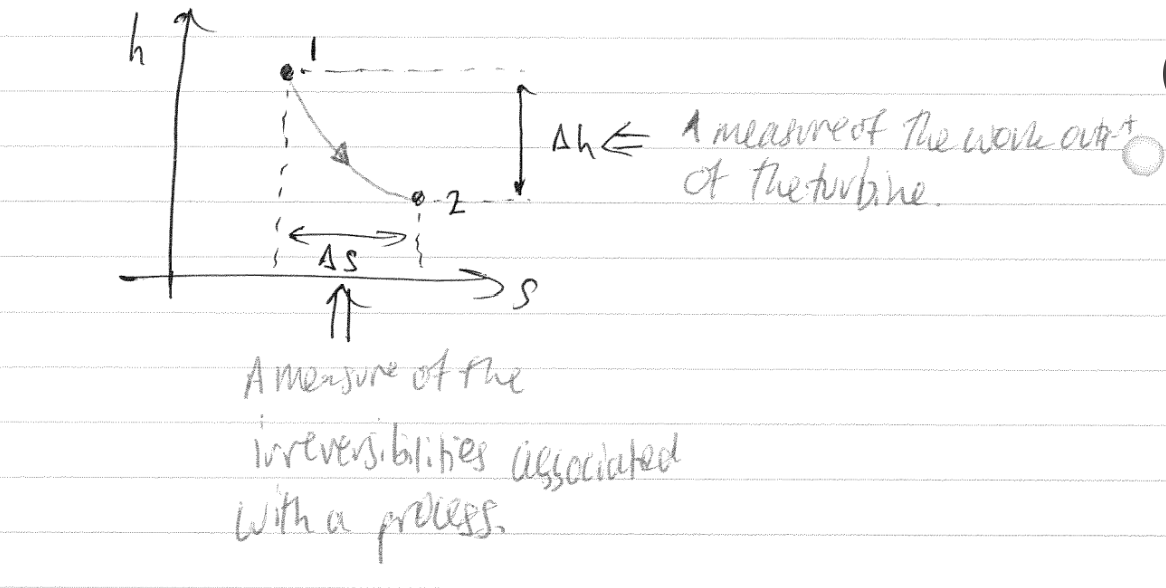
\includegraphics[width = \textwidth]{../img/MollierDiagram}
  \caption{Mollier Diagram}
\end{figure}
\subsection{T-S diagram of the Carnot cycle}
The Carnot cycle is made up of two, reversible isothermal CT = constant S processes and two isentropic (adiabatic and S = constant) processes. These four processes form a rectangle on the T-S diagram. 
\begin{figure}
  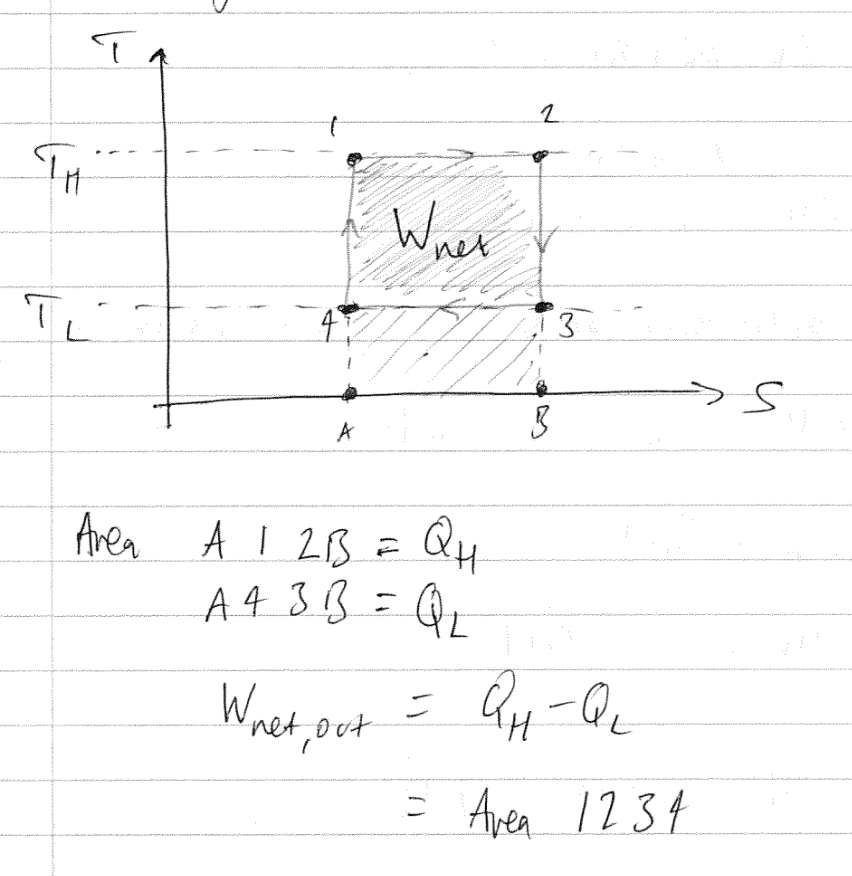
\includegraphics[width = \textwidth]{../img/TSDiagramCarnotCycle}
  \caption{T-S diagram for the Carnot cycle}
\end{figure}
\subsection{The Tds relations}
The first law states:
\[ \Delta E = \Delta U + \Delta KE + \Delta PE \]
For closed systems that are stationary, \( \Delta KE = \Delta PE = 0 \) therefore, 
\begin{align*}
  \Delta E &= \Delta U\\
  \Delta U &= \Delta Q + \Delta W (+ \Delta E_{mass} = 0)\\
  \Delta U &= \Delta Q + \Delta W\\
  \Delta U &= Q_{\textrm{net in}} - W_{\textrm{net out}}
\end{align*}
In differential form and for: a simple compressible substance, an internally reversible process,
\[ dU = SQ_{\textrm{int rev}} - SW_{\textrm{int rev out}} \]
But \( SQ_{\textrm{int rev}} = T dS \) and \( SW_{\textrm{int rev out}} = PdV\) thus,
\begin{align*} 
  dU &= TdS - PdV\\
  TdS &= dU + PdV \ (\si{\kilo\joule})\\
  Tds &= du + Pdv \ (\si{\kilo\joule\per\kg})
\end{align*}
\end{document}